\documentclass[
    a4paper,
    12pt,
    oneside
]{report}

% Import packages
\usepackage{graphicx}
\usepackage{subfigure}
\usepackage{amsmath}  % Replaced latexsym with amsmath for symbols and mathematical operations
\usepackage[utf8]{inputenc}
\usepackage[english]{babel}
\usepackage{pdfpages}
\usepackage[
    backend=biber,
    style=ieee
]{biblatex} % IEEE style citations
\usepackage{url}
\usepackage[T1]{fontenc}
\usepackage{float}
\usepackage{palatino}
\usepackage{color}

\setlength{\doublerulesep}{\arrayrulewidth}
\setlength{\textwidth}{16cm}
\setlength{\textheight}{24cm}
\setlength{\hoffset}{-1.7cm} 
\setlength{\voffset}{-1cm}
\setlength{\topmargin}{-0.5cm} 
\setlength{\footskip}{27pt}

\renewcommand{\baselinestretch}{1.3}
\linespread{1}

\usepackage{titlesec}
\titlespacing*{\chapter}{0pt}{-1\baselineskip}{1\baselineskip}
\titlespacing*{\section}{0pt}{\baselineskip}{0pt} 

\usepackage{fancyhdr}

\fancypagestyle{noheadrule}{
    \fancyhf{}
    \renewcommand{\headrulewidth}{0pt}
    \renewcommand{\footrulewidth}{0.5pt}
    \fancyfoot[L,LO]{\textit {FINAL PROJECT PROPOSAL}}
    \fancyfoot[R,RO]{\bfseries\thepage}
}

% Add bibliography file to document
\addbibresource{biblio.bib}

\begin{document}

% Cover
\begin{titlepage}
    \centering
    % \vspace*{1cm}

    {\LARGE \textbf{Final Project I}}\\[1cm]
    {\Huge \textbf{Collective Transport using Decentralised Swarm Robotics}}\\[1cm]

    
\includegraphics[width=0.4\textwidth]{assets/images/ise_logo.png}\\[1cm]
    
    \textbf{Submitted to the}\\[0.1cm]
    Project Committee appointed by the\\
    \textbf{International School of Engineering (ISE)}\\
    Faculty of Engineering, Chulalongkorn University\\[1cm]

    \textbf{Project Adviser}\\[0.1cm]
    Asst.Prof.Paulo Fernando Rocha Garcia, Ph.D.\\[1cm]

    \textbf{Submitted By}\\[0.5cm]
    \begin{tabular}{rl}
        6438067021 & Nattadon Tangsasom \\
        6438075021 & Ting-Yi Lin \\
        6438079621 & Tinapat Limsila \\
        6438118421 & Noppawan Srikhirin \\
        6438187721 & Mehul Sharma \\
    \end{tabular}\\[1cm]
    2/2024: 2147417 Final Project II\\
    Robotics and Artificial Intelligence Engineering (International Programme)\\
    International School of Engineering (ISE) Faculty of Engineering, Chulalongkorn University

\end{titlepage}


\thispagestyle{empty}
\pagenumbering{roman} \setcounter{page}{1}
\setcounter{secnumdepth}{11}
\setcounter{tocdepth}{3}
\renewcommand{\chaptermark}[1]{\markboth{Chapter ~\thechapter~:~#1}{}}
\fancyhf{}
\fancyhead[R,RO]{\bfseries\leftmark}
\fancyfoot[L,LO]{\textit {FINAL PROJECT PROPOSAL}} 
\fancyfoot[R,RO]{\bfseries\thepage}
\fancypagestyle{plain}{
    \fancyhead{}
    \renewcommand{\headrulewidth}{0pt}
} 
\pagestyle{fancy}
\selectlanguage{english}
{\linespread{.8}\tableofcontents}
\newpage
\pagenumbering{arabic}
\titlespacing{\chapter}{0cm}{1cm}{2cm}

% Chapters
\chapter{Introduction}

\paragraph*{}
This progress report aims to highlight the progress of our final project, \textbf{Collective Transport using Swarm Robotics}, with the evaluating criteria being the team individual contributions, as well as our pace in comparison to the ideal schedule. The ideal schedule can be represented by the project Gantt Chart (Figure \ref{fig:gantt_chart}).

\paragraph*{}
According to Figure \ref{fig:gantt_chart}, we are exploring three major sub-tasks during this iteration of the project schedule. These three tasks are: \textbf{Communication in the Swarm} (Task 1.1), \textbf{Object detection using Computer Vision} (Task 1.2), and \textbf{Simple Simultaneous Localization and Mapping} (Task 1.3). These tasks are planned to span for the entire month of September. Two team members, one team member, and two team members are assigned to each task, respectively.

\begin{figure}[H]
    \centering
    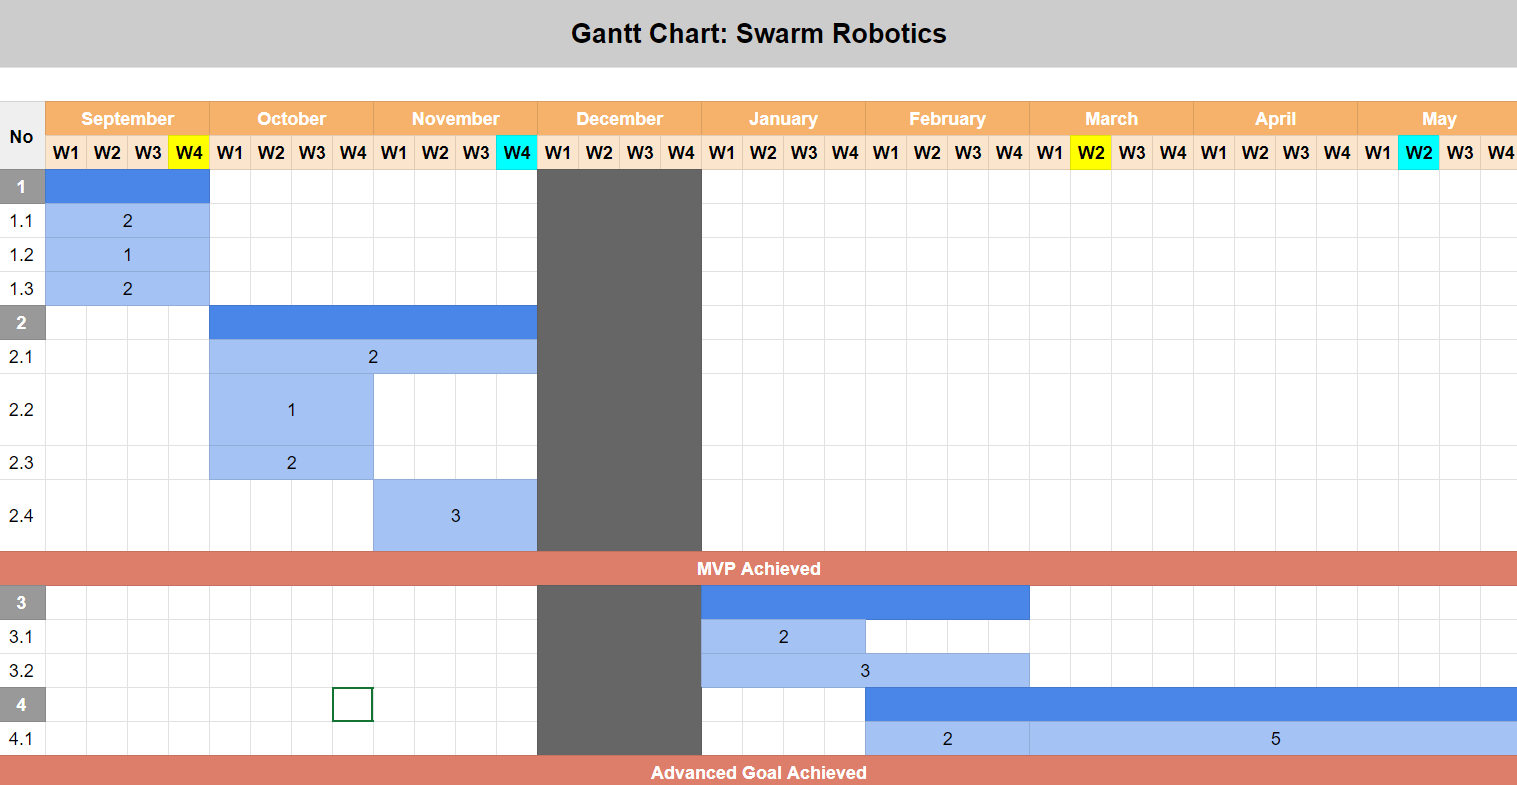
\includegraphics[width=1\linewidth]{progress_report_1/assets/images/introduction/gantt_chart.png}
    \caption{Project Gantt Chart}
    \label{fig:gantt_chart}
\end{figure}

% \chapter{Communication}

\paragraph*{}
This chapter details the exploratory results for the sub-task \textbf{Communication in the Swarm}. This task has been tackled under the assumption that the \textit{swarm fleet are capable of object detection}, which is a necessary premise to parallelize the workload as another group member is working on it. Some other vital constraints include:

\begin{itemize}
    \item \textbf{Robots are stationary} \\
    This is assumed because we can temporarily exclude motor control for simplicity
    \item \textbf{Robots are on fixed coordinates configured by the user} \\
    This is assumed because robots can communicate their coordinates to other fleet members and the assumption offers an easy method to check for the correctness in their communication.
    \item \textbf{Start with 5 robots during simulation} \\
    This constraint is to minimize the complexity in the environment
\end{itemize}

\paragraph*{}
After thorough consideration and evaluation, the best simulating environment for this specific communication task is Webots from Cyberbotics. Webots provide the PROTO mechanism for developers to build and reuse complex objects. This allows us to simulate and test our assumptions upon pre-built objects, such as 
TurtleBot. 

\begin{figure}[H]
    \centering
    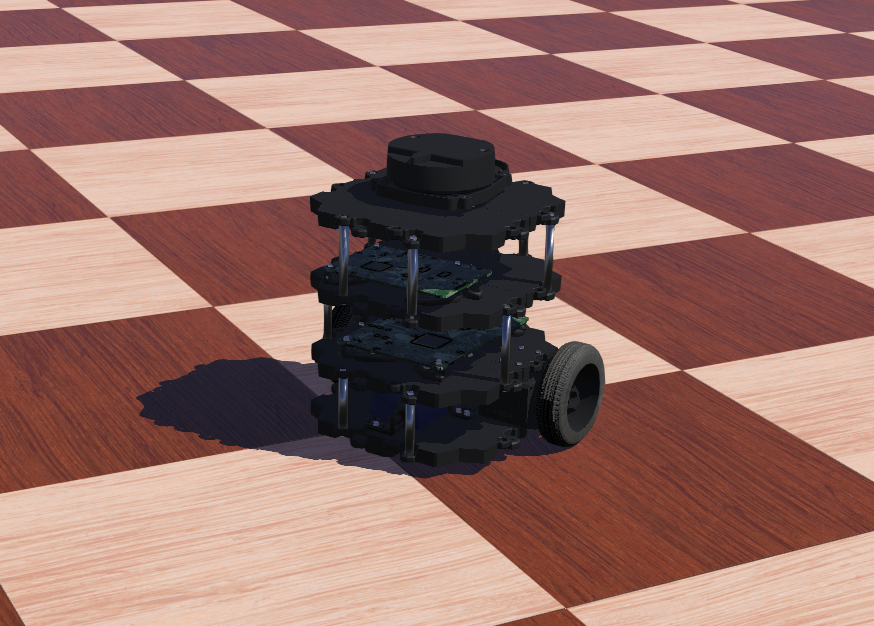
\includegraphics[width=0.4\linewidth]{assets/images/communication/environment/turtlebot.png}
    \caption{TurtleBot 3 Burger in Webots}
    \label{fig:turtlebot}
\end{figure}

In webots, the version of the TurtleBot given in the PROTO nodes is the Burger model of the third version of the TurtleBot robot Figure \ref{fig:turtlebot}.  Moreover, the TurtleBot has two functioning motors and a 360-degree distance sensor, allowing it to do simple navigation. However, using TurtleBot alone is inadequate to simulate the communication framework. Therefore, three more basic nodes are added to the TurtleBot object, which are the following: Firstly, the GPS node (Figure \ref{fig:GPS}), this module is installed to obtain the robot's position in the simulated world. This direct approach is used because the localization and mapping process is not accounted for in this testing. Secondly, the Emitter node (Figure \ref{fig:Emitter}), this module is added to the robot to model a broadcast behavior. Additionally, Webots allows the developer to configure the properties of the Emitter Class; for instance, the emission range. Thirdly, the Receiver node (Figure \ref{fig:Receiver}), this module is connected as an accompaniment to the Emitter Class, because the Emitter node does not support both emitting and receiving functionalities. The receiver listens for incoming data packets and appends them to the tail of a queue. Moreover, incoming data packets will be discarded if the receiver's buffer size is exceeded. With all the

\begin{figure}[!htb]
    \minipage{0.32\textwidth}
        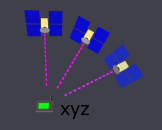
\includegraphics[width=\linewidth]{assets/images/communication/devices/gps.png}
        \caption{GPS node}\label{fig:GPS}
    \endminipage\hfill
    \minipage{0.32\textwidth}
        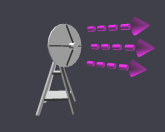
\includegraphics[width=\linewidth]{assets/images/communication/devices/emitter.png}
        \caption{Emitter node}\label{fig:Emitter}
    \endminipage\hfill
    \minipage{0.32\textwidth}%
        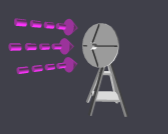
\includegraphics[width=\linewidth]{assets/images/communication/devices/receiver.png}
        \caption{Receiver node}\label{fig:Receiver}
    \endminipage
\end{figure}

\paragraph*{}
The main approach to communication in the swarm would be to gain awareness over robotic members in the swarm system and finding consensus within the swarm before any further follow-up actions are taken. In case of an object getting detected, the first robot that detects the object would act as the task master, supplying other robots in the swarm with the object's coordinates. Consensus is essential for this use case because every swarm members have to agree on the object detection before any actions. Therefore, we are utilizing modes to build a central template code to operate the swarm. There are two main modes for the swarm: \textbf{Idle} mode and \textbf{Consensus} mode.

\paragraph*{}
The \textbf{Idle} mode entails the period where fleet members are setting themselves up by communicating their \textbf{identifiers} and their \textbf{coordinates}, which the receivers store as internal dictionaries. Figure \ref{fig:idle_mode} displays the functional instance where the turtlebots in the environment are aware of other members and their respective coordinates and test-print them on console.

\begin{figure}[H]
    \centering
    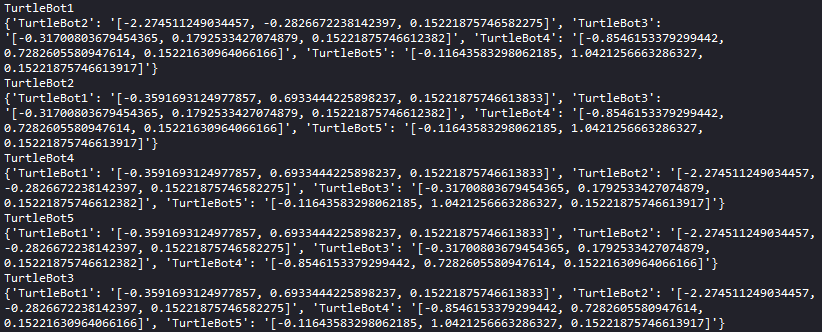
\includegraphics[width=1\linewidth]{assets/images/communication/outputs/idle_mode.png}
    \caption{Idle Mode}
    \label{fig:idle_mode}
\end{figure}

\paragraph*{}
The \textbf{Consensus} mode occurs when an object is "detected" by any of the swarm members. After the detection, the robot which identifies the object will switch its mode to Consensus and save the object's coordinates. Consequently, it will communicate to other members of the present object, readying them for any subsequent actions. In this test case, a set of object coordinates is manually supplied to one of the members after four seconds. Figure \ref{fig:consensus_mode} shows \textit{TurtleBot2}, a member in the environment, receiving the set of coordinates and communicating to the swarm that it is the task master and the location of the object, thereby bumping other robots' modes to Consensus mode.

\begin{figure}[H]
    \centering
    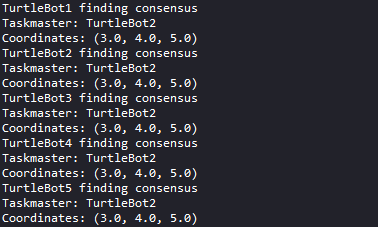
\includegraphics[width=0.6\linewidth]{assets/images/communication/outputs/consensus_mode.png}
    \caption{Consensus Mode}
    \label{fig:consensus_mode}
\end{figure}

\paragraph*{}
This approach can be improved by planning for worst-case-scenarios in advance. To expand further, this can be from preventing any race conditions occurring from the consensus mode, and including an extra verification step after communication. However, a potential challenge with the verification step is that robotic communication is extensive; having additional communication demands should be in balance with the available resources the robots allow.

\paragraph*{}
Additionally, the \textbf{application layer} is currently sending and receiving:

\begin{itemize}
    \item Robot's identifier
    \item Robot's coordinates
    \item Object coordinates
\end{itemize}

We will potentially require more information to be transmitted with additional requirements from other modules, which is another area for further improvements.

% \chapter{Object Detection}

\paragraph*{}
The object detection system initially developed in the previous semester successfully detected a yellow cylinder, generated a bounding box around it, aligned the box’s center with the camera frame, and measured the distance between the robot and the object using the camera’s focal length. However, this implementation relied on the assumption that the cylinder’s dimensions were known, and LiDAR had not yet been integrated. Additionally, the scope of object detection was refined from hexagonal prisms and cubes to cylinders to eliminate the need for pose estimation and edge detection, which would otherwise introduce additional computational complexity for dynamic object grasping.

\paragraph*{}
In transitioning to real-world implementation, several modifications were made to the object detection workflow. The system now identifies three distinct objects: a yellow, a blue, and a red cylinder, each differing in size. At this stage, only a single object is placed in the arena at a time, with detection based primarily on colour. Once detected, the system generates a bounding box around the object, and its distance and size are measured using an S3 RPLiDAR. To enhance accuracy, multi-sensor fusion between the camera and LiDAR is employed. By leveraging the camera’s horizontal field of view (FOV), the system maps the bounding box’s pixel range to the corresponding angle and retrieves the appropriate LiDAR data based on the robot’s odometry.

\paragraph*{}
The current implementation has successfully demonstrated the ability to detect objects based on color while filtering out reflections from the floor. Initial testing was conducted under controlled lighting conditions, including illumination from the left, right, front, and back. The presence of vibrations caused by the camera mount during movement did not significantly affect detection performance. However, at this stage, accuracy assessments are still based on visual inspection, and further validation will be conducted once the model undergoes proper calibration with the sensors. Overall, progress remains on schedule and aligns with the expected timeline, with each milestone being achieved as planned.

\paragraph*{}
In measuring distance and size, image distortion remains a key factor influencing accuracy, as the system must correctly map the detected object’s bounding box angle to real-world coordinates. Since the object’s height does not contribute to measurement calculations, vertical calibration data from the camera has been omitted. Additionally, the top 30 degrees of the camera frame is cropped to remove potential noise and prevent false detections of unintended objects or individuals outside the arena.

\paragraph*{}
One of the primary challenges encountered in this phase is object occlusion, where multiple objects appearing in the frame can lead to overlapping bounding boxes. In such cases, the robot is required to reposition itself to separate the detected objects and ensure accurate size measurements without interference. Another challenge is ensuring reliable color detection under varying lighting conditions, as different light sources and angles can affect how the camera perceives object colors. Additionally, image distortion presents difficulties in mapping the bounding box to the correct position in relation to the LiDAR data. These obstacles are being addressed through careful calibration, adjustments in object positioning, and improvements to the detection algorithm to enhance its robustness against occlusion and lighting variations.

\paragraph*{}
To meet the minimum viable product (MVP) requirements, the initial implementation is limited to detecting a single object within the arena. The system must be capable of generating a bounding box, measuring both distance and angle, and determining the object's size using LiDAR. Once these fundamental objectives are achieved, the next phase of testing will involve detecting multiple objects within a single frame while handling occlusion through coordinated robot movement.

\paragraph*{}
Further testing will focus on optimizing the model and evaluating its accuracy under different conditions. The model will first be validated under the MVP scenario, dealing with only one object, before advancing to a multi-object setting with occlusion management. To assess distance measurement accuracy, objects will be placed at 0.5, 1, and 3 meters from the robot, allowing evaluation of the alignment between LiDAR and camera data. Additionally, eight different lighting conditions will be introduced by positioning the light source at varying angles to examine the robustness of the color detection model under diverse illumination environments.

% \chapter{Choice of SLAM}

\paragraph*{}
In our last progress report we mentioned that we had a very basic implementation of SLAM working. This however is only true in some aspects. While we do have a basic implementation of localisation, we do not currently have the ability to do simultaneous mapping of an unknown environment which was a mistake on our part. In the following weeks, we first attempted to implement SLAM through the use of ROS2 so we could easily access SLAM libraries like gmapping and cartographer . We specifically used ROS2 with the turtlebot3burger all integrated together in webots. However; we faced problems when it came to the communication between ROS2 and the simulation due to our limited experience with the aforementioned software. We then decided to pursue a SLAM option that does not depend on ROS such as EKF SLAM and Graph SLAM. EKF SLAM initially seemed familiar to us as we recently learnt the Kalman filter. However; we decided to go with graph SLAM for numerous reasons. Graph SLAM is more accurate than EKF SLAM because it performs global optimization by maintaining a graph of all robot poses and measurements, allowing for efficient correction of accumulated errors, especially during loop closure when the robot revisits known locations. This could be especially helpful in our project since our robots after placing the object in its desired location will be coming back to the main map. Unlike EKF SLAM, which uses linearization and only updates the current pose, Graph SLAM adjusts the entire trajectory and map, minimising drift and non-linearities. 
% \chapter{Hardware}

\paragraph*{}
Due to the predicted cost of hardware, we decided to ask a local Chulalongkorn University robotics club for one of their swarm robots, particularly the robot used in a previous RoboCup soccer competition. While the electronics in these robots are outdated, the motors remain exceptional, as they are Maxon motors, known for their reliability, efficiency, and speed. Hiveground, one of our project supporters, has also agreed to provide us with another identical robot, as one of the founders is an alumnus of the EIC. At the time of writing, we currently have two identical robots in our possession.

\begin{figure}
    \centering                 
    \includegraphics[width=0.4\linewidth, angle=270]{assets/images/hardware/robobot.JPG}
    \caption{One of the robots obtained from EIC Chula, RoboCup}
    \label{fig:robobot}
\end{figure}

\paragraph*{}
The Maxon motors in both robots are arranged in an X layout, paired with high-quality omnidirectional wheels. However, due to a lack of use over the past decade, the rubber on the wheels has decayed. Given the custom nature of these wheels, we will 3D print new rubber O-rings to replace the old ones. Omnidirectional wheels are ideal for this case due to their ability to provide smooth and precise multi-directional movement, which is crucial for achieving accurate and agile manoeuvres in swarm robotics applications, allowing the robots to navigate and collaborate effectively in complex environments.
\paragraph*{}
The next step involves testing the motors, including their encoders, to evaluate the accuracy, power, and torque of the current setup. Our goal is to determine whether these motors can perform adequately as servomotors for precise control and calculations. For this purpose, we will use an Arduino to control the motors during testing.
\paragraph*{}
In terms of schedule, we are currently ahead of the planned timeline for the hardware development stage, giving us some flexibility for further testing and refinement.

\paragraph*{}
We have encountered issues with reusing old motors and robots from RoboCup Soccer. The Hall effect sensor and the optical sensor have worn out. To address this, we designed and 3D-printed a bracket to mount the Maxon EC 45 Flat motor along with the AS5600 magnetic encoder. We are currently testing the motor to achieve closed-loop control. The motors in the robot are custom-made, and we do not know the number of pole-pairs, making calibration more challenging. 

Initially, we used the SimpleFOCmini V1.0 drive board, leveraging the SimpleFOC library for testing. However, after further evaluation, we have decided to transition to the XDrive by Makerbase with ODrive firmware. This decision was made due to the superior support provided by the ODrive community and its extensive documentation, which offers better reliability and ease of integration into our project. The XDrive with ODrive firmware will replace the SimpleFOC solution and be used for achieving precise closed-loop control of the motors.
\begin{figure}
    \centering
    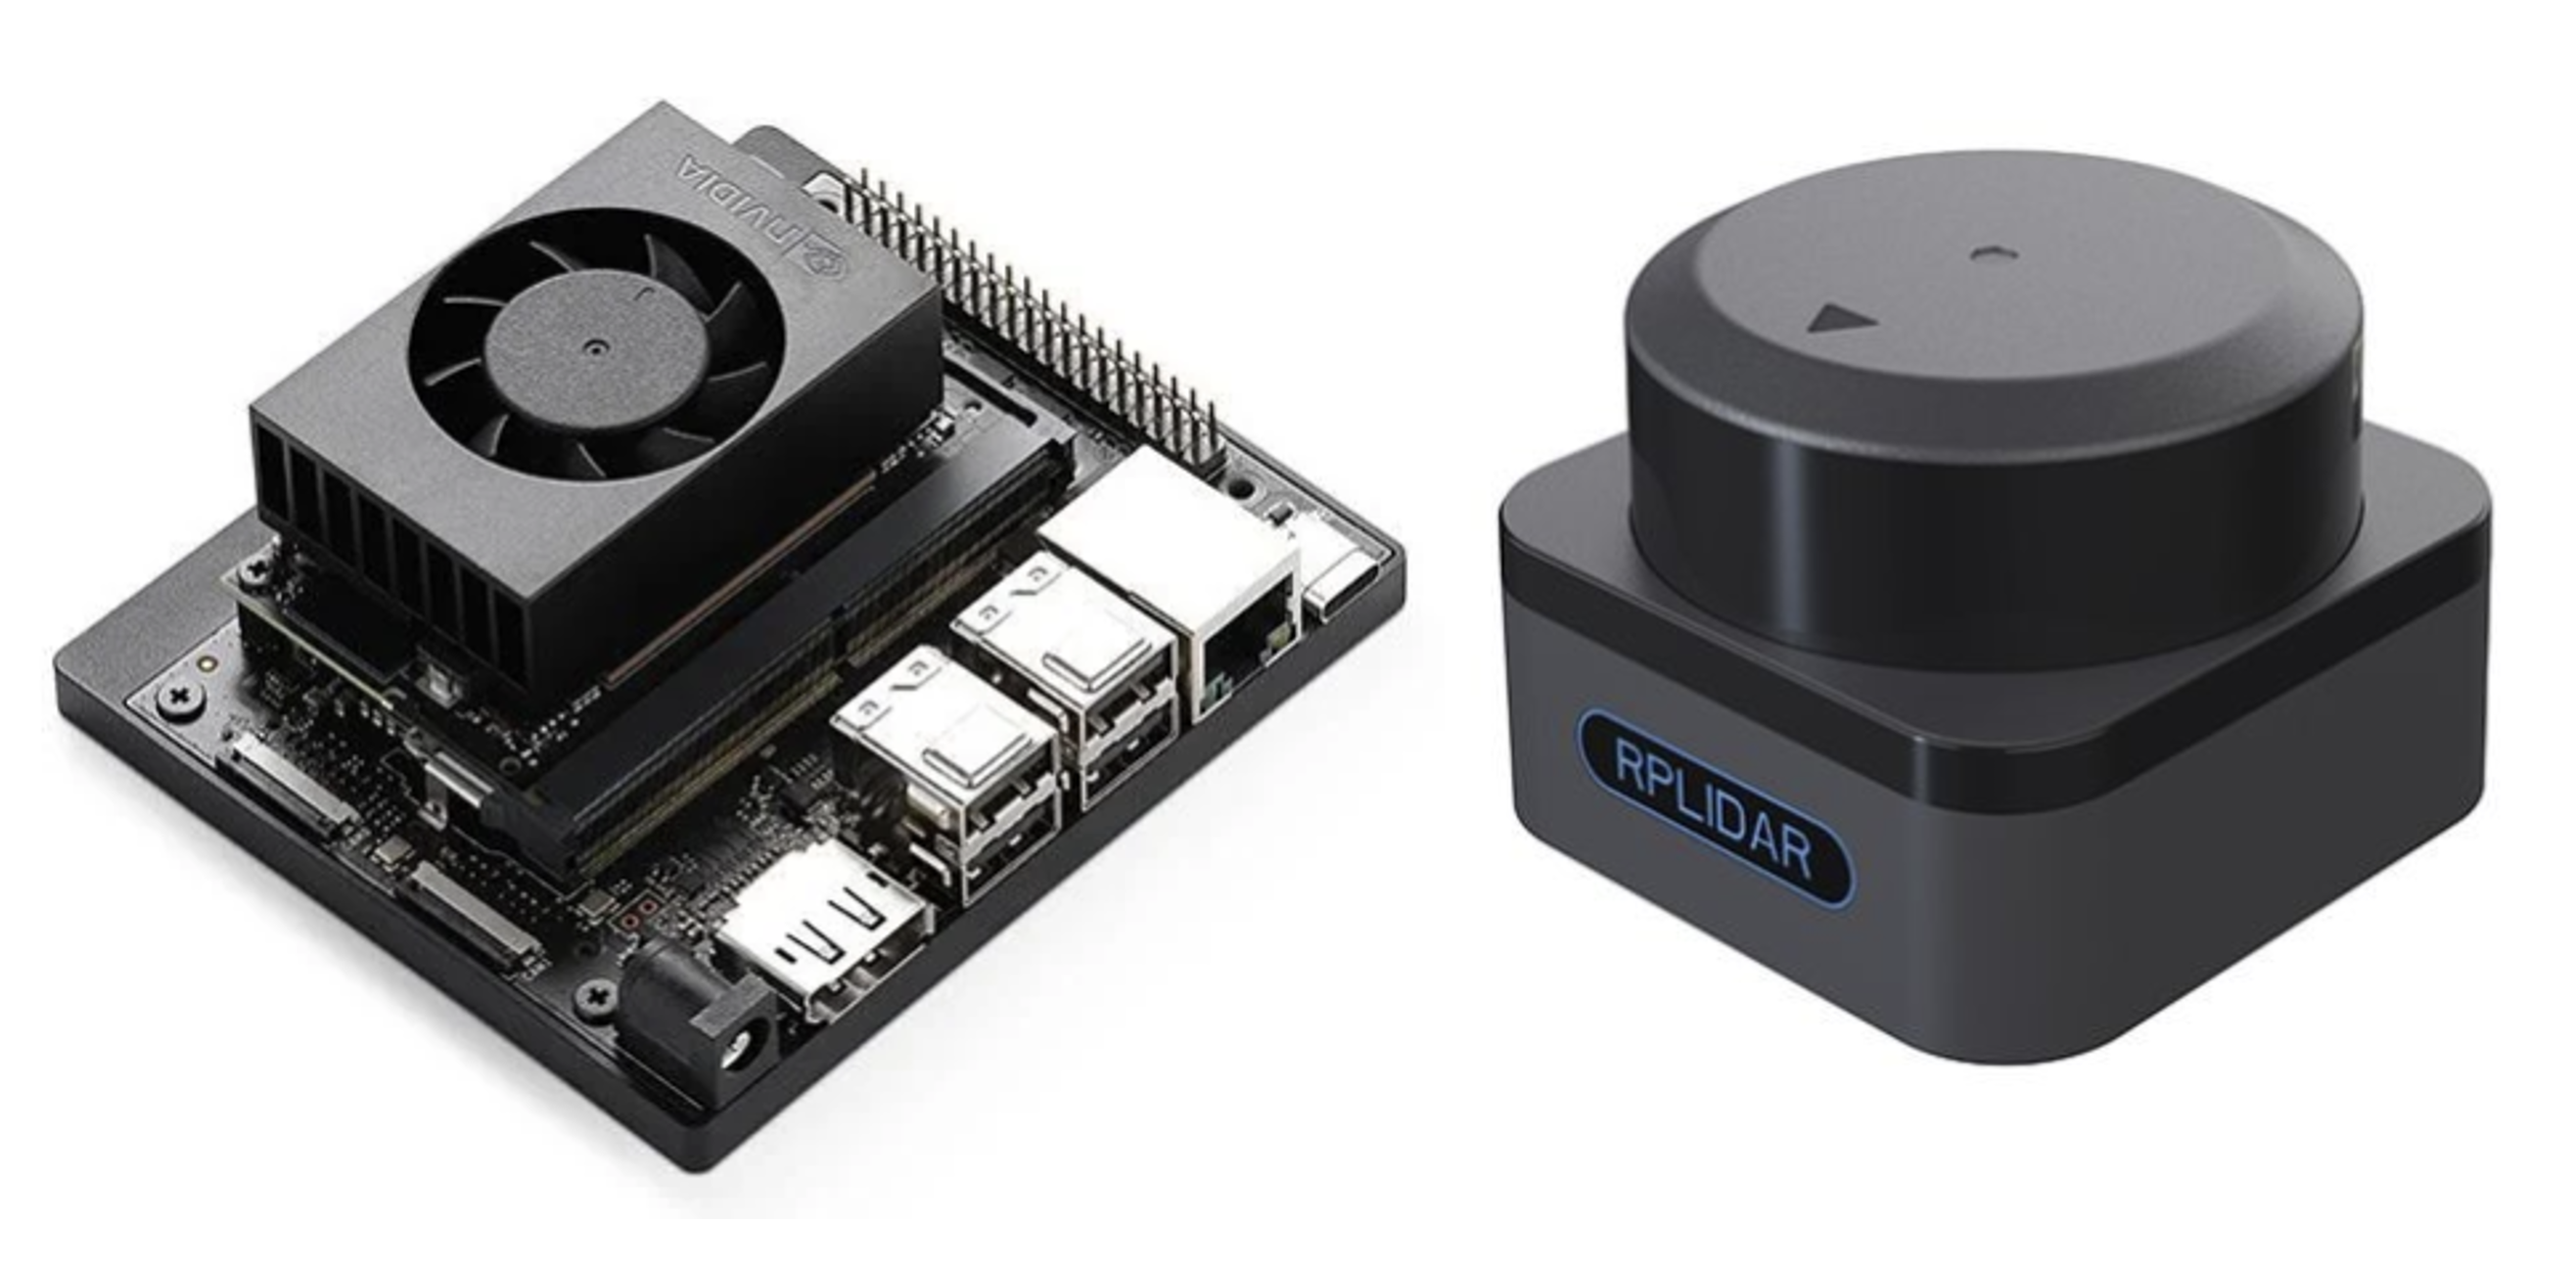
\includegraphics[width=0.5\linewidth]{midpoint_report//assets//images//hardware/JetsonNano+RPLiDAR.png}
    \caption{Image of the Jetson Nano Orin(left) and RPLiDAR S3 360(right)}
    \label{fig:enter-label}
\end{figure}
\paragraph*{}
The next step, after achieving closed-loop control using XDrive with ODrive firmware, is to purchase additional motor drivers and control all four wheels. This will allow us to properly drive the X-Drive omnidirectional system using the Jetson Nano (see \ref{fig:hardware-arch})), which will then be abstracted to operate under ROS.
\begin{figure}
    \centering
    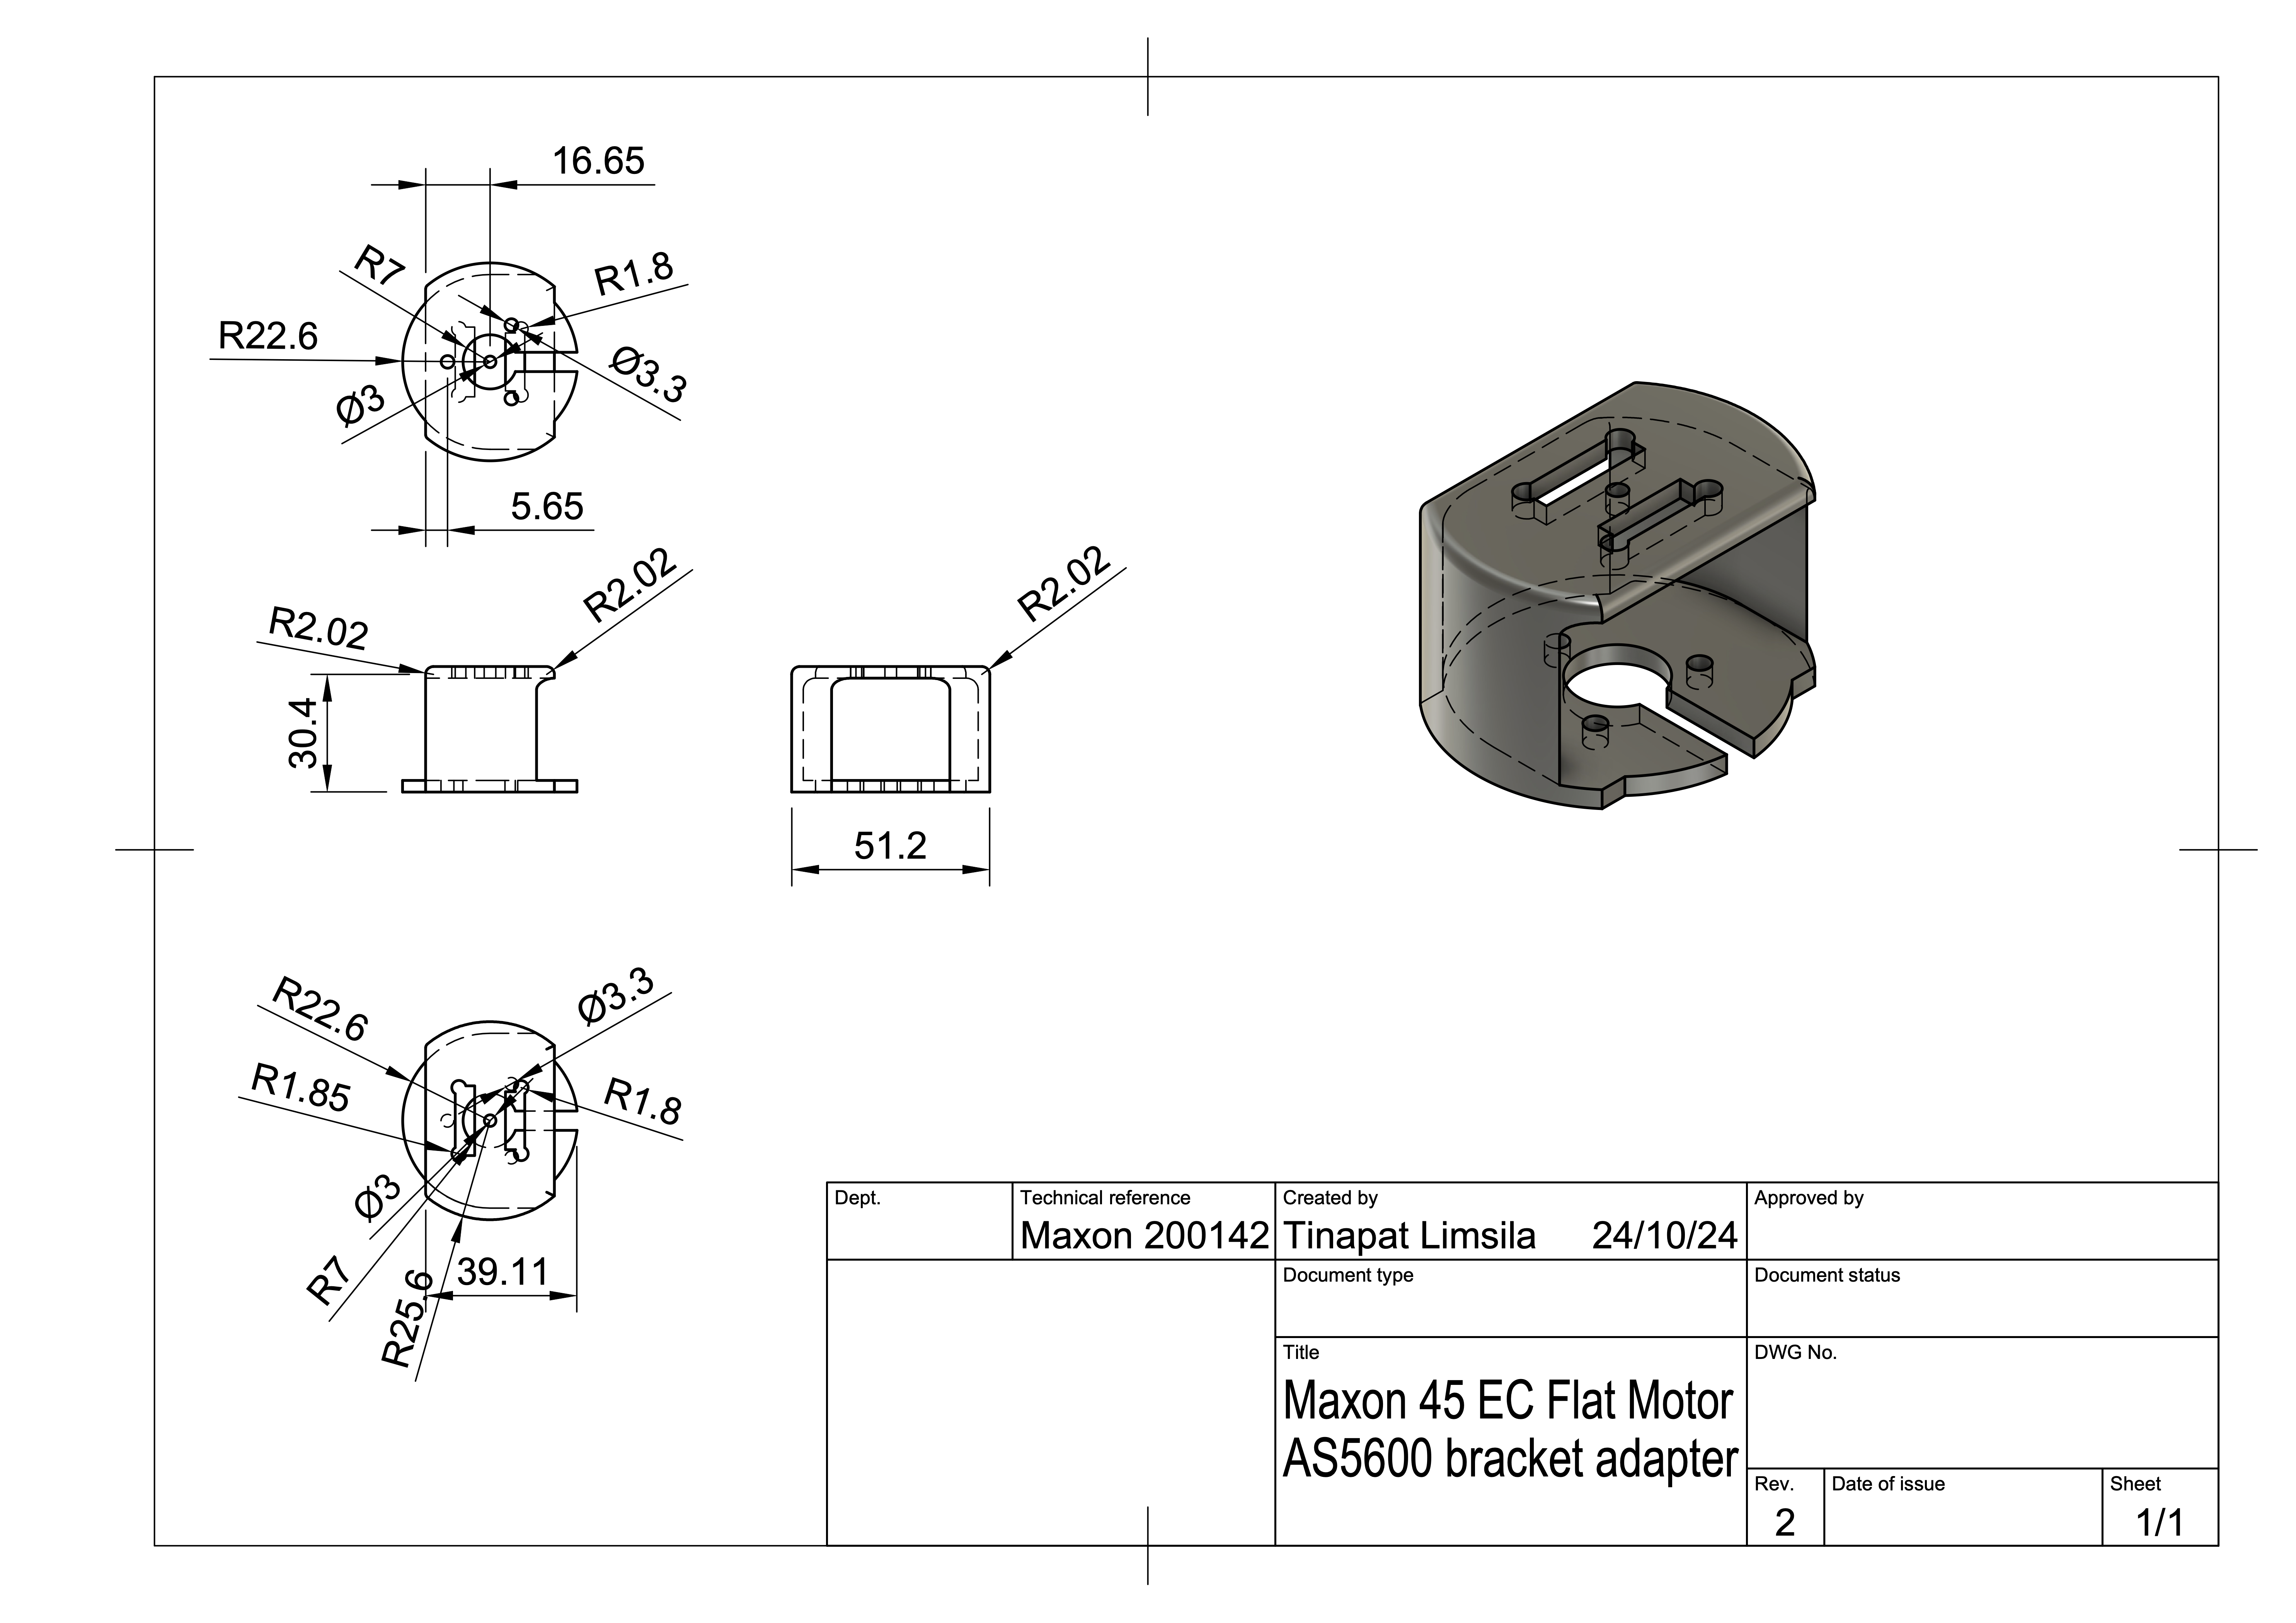
\includegraphics[width=1\linewidth]{assets/images/hardware/Maxon 45 EC Flat Motor AS5600 bracket adapter Drawing v1.png}
    \caption{CAD drawing of the bracket for the Maxon 45 EC Flat motor and the Magnetic Encoder for AS5600}
    \label{fig:real-single-robot}
\end{figure}

\begin{figure}
    \centering
    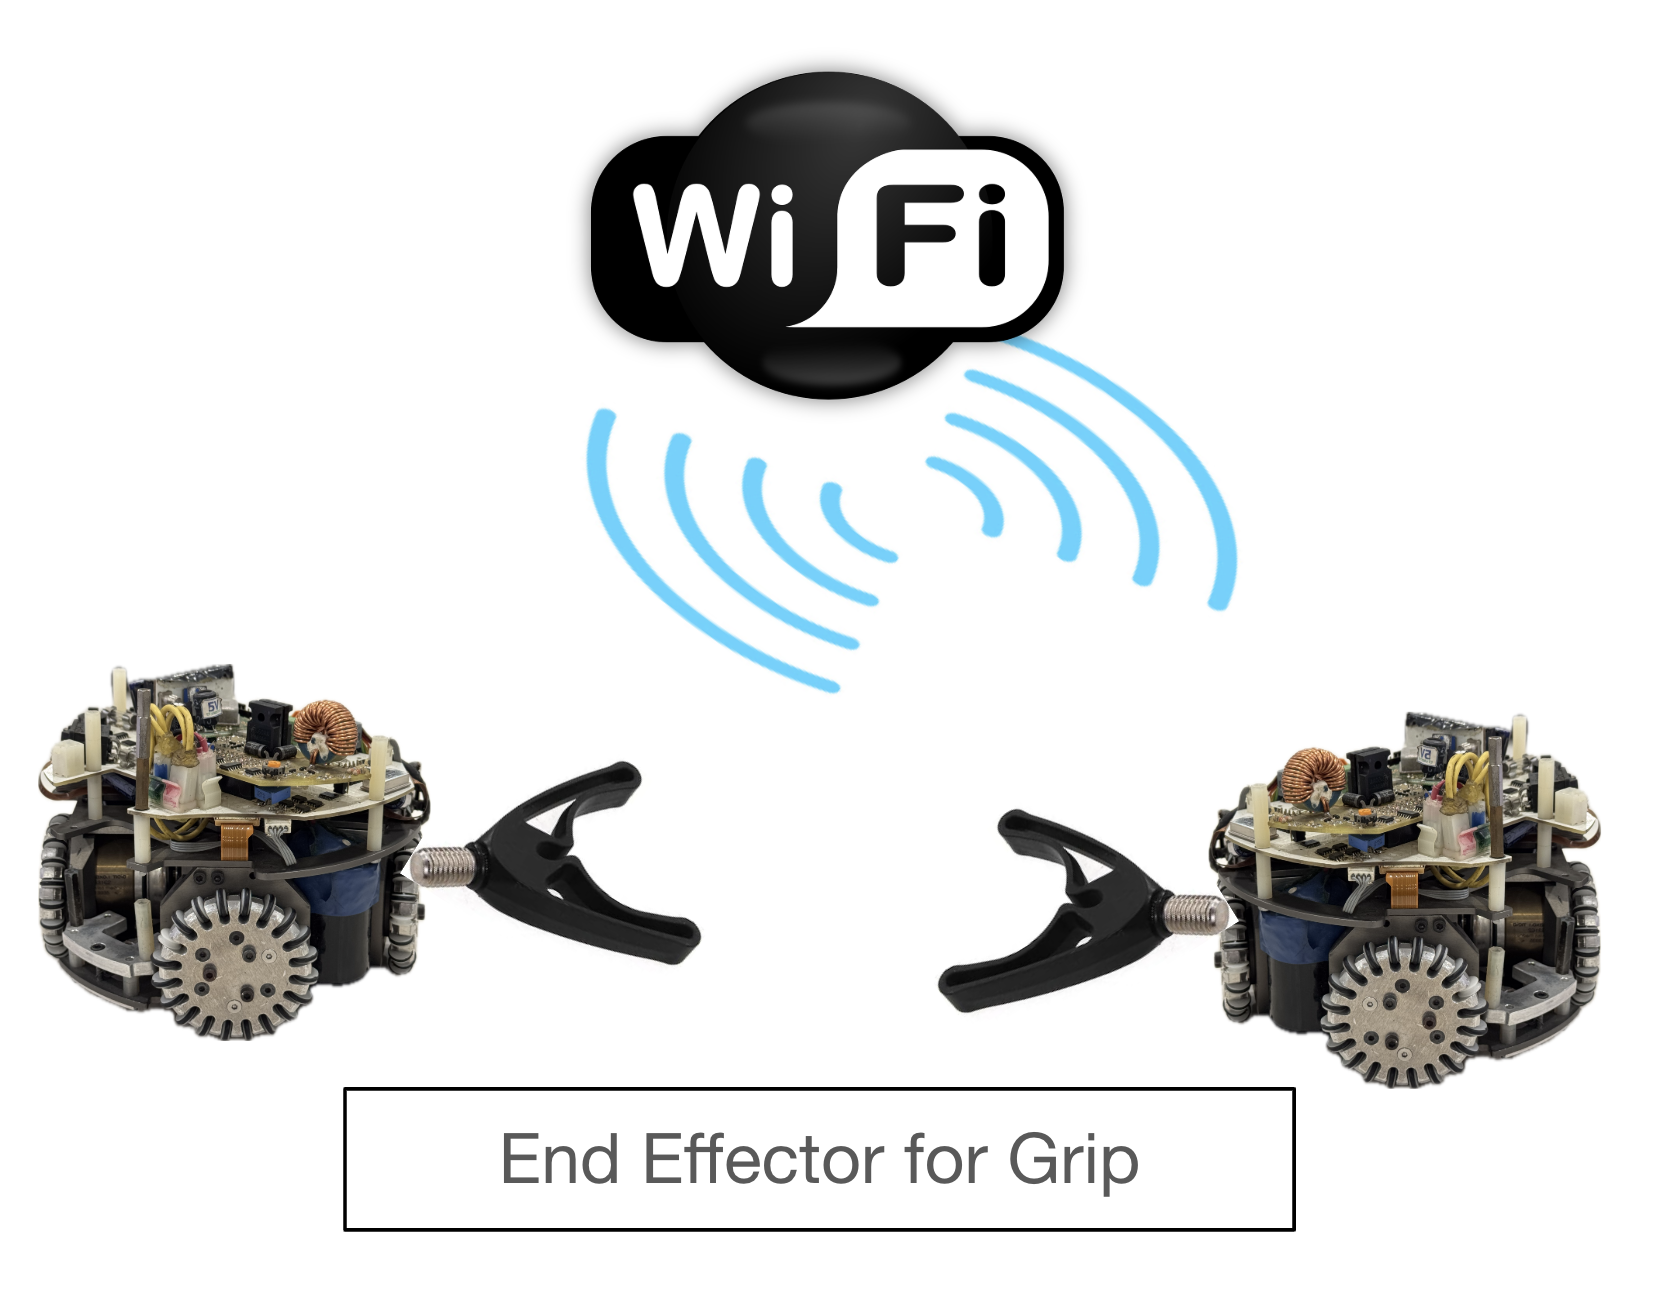
\includegraphics[width=0.5\linewidth]{assets/images/hardware/endeffector.png}
    \caption{Image of the two swarm robot with end effectors with communication via WiFi}
    \label{fig:effector-2-robot}
\end{figure}
\begin{figure}
    \centering
    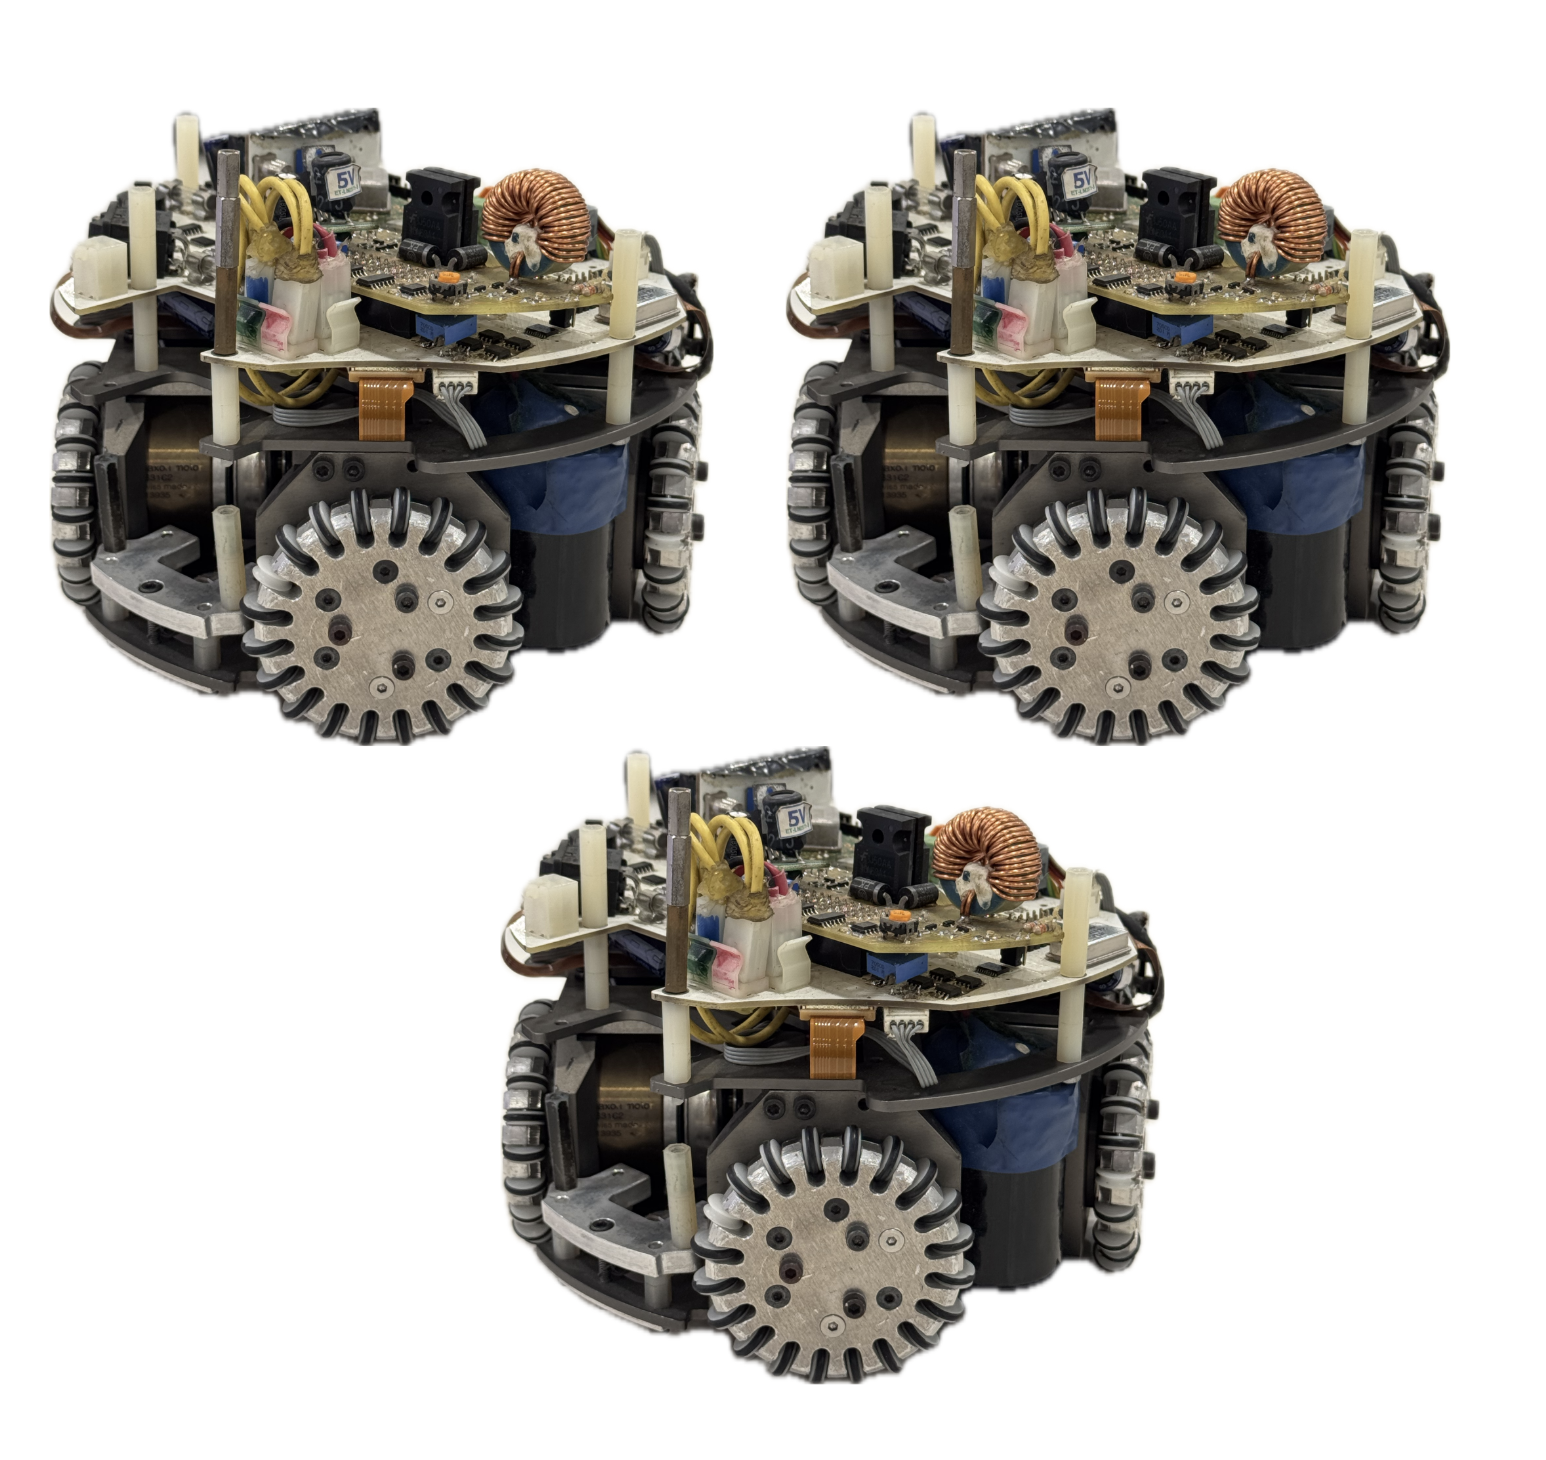
\includegraphics[width=0.5\linewidth]{assets/images/hardware/3swarmrobots.png}
    \caption{Image of the 3 acquired swarm robot pre-modification}
    \label{fig:3-robot}
\end{figure}\begin{figure}
    \centering
    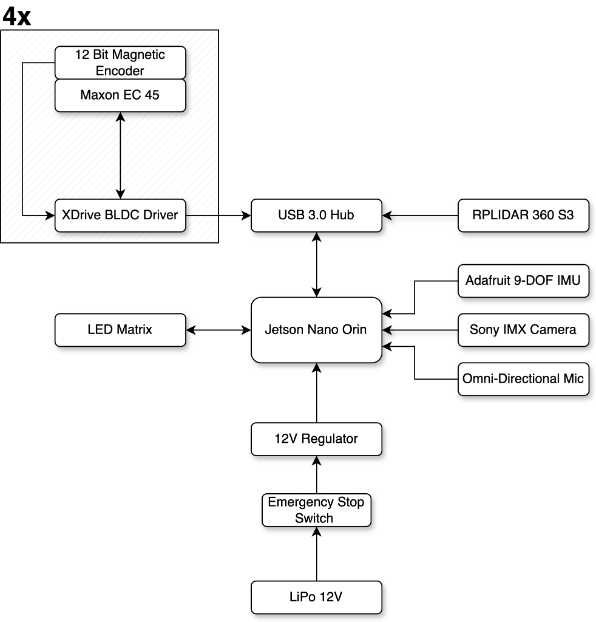
\includegraphics[width=0.75\linewidth]{midpoint_report/assets/images/hardware/hardware-architecture.png}
    \caption{Image of a the hardware architecture and I/O of the system}
    \label{fig:hardware-arch}
\end{figure}

Our hardware in Figure \ref{fig:hardware-arch}, will have safety features such as microphones and an emergency stop button if the robot has software malfunctions. The LED matrix will be the indicator for taskmaster. RPLiDAR 360 S3 will be used for Graph SLAM with the ROS interface package provided. 

\chapter{Conclusion}

\paragraph*{}
Swarm communication has been successfully implemented using a decentralized peer-to-peer architecture facilitated by socket communication. This approach was selected for its low latency and reliability, both of which are essential for real-time data exchange among robots. A three-way handshake mechanism was incorporated to ensure message delivery integrity, along with a consensus algorithm to resolve simultaneous object detection and taskmaster assignment conflicts. With coordinate streaming, dynamic path planning, and task execution now fully integrated, the communication system provides a solid foundation for coordinated swarm behavior, enabling seamless transitions between detection, planning, and movement phases.

\paragraph*{}
Additionally, the object detection system utilizing multi-sensor fusion of the camera and S3 RPLiDAR accurately measures relative distance, relative angle, and estimated width, aided by the variation factor function. This function yields an error margin of 1 centimeter for cylinders with diameters of 16 and 20 centimeters. The model was also tested with objects of different sizes, specifically a cylinder with a diameter of 12 centimeters, resulting in a slightly higher error margin of 2 centimeters. Overall, the object detection component was completed within the expected timeline.

\paragraph*{}
For SLAM we will continue making our own graph SLAM but will work on SLAM Toolbox temporarily. For odometry, we will continue testing and publish results soon.

\paragraph*{}
Meanwhile, the development and testing of our holonomic X-Drive robot have progressed significantly. The robot’s base and structural components were 3D printed using PLA, but to improve durability and stability, key parts such as the baseplate, shaft, wheels, and flange coupler will be upgraded to acrylic and stainless steel. The robot utilizes Dynamixel AX-12W motors for enhanced back-drivability, controlled through a custom ROS 2 package that applies a Jacobian matrix transformation for motion control. Transitioning from the older Maxon BLDC motors has streamlined development, allowing us to focus on software for coordinated multi-robot operation. The successful integration of the teleop keyboard package in ROS 2 Humble has demonstrated holonomic movement, paving the way for further improvements in geometry and performance optimization.

\paragraph*{}
For the next phase of our project, we will complete the tasks that have yet to be completed during the previous iteration and move towards a complete swarm. This includes completing the hardware requirements, considering movement after gripping, as well as testing and evaluation. Additionally, we will proceed with other tasks as scheduled in the Gantt Chart to ensure all project milestones are met.


% Bibliography
\nocite{*}
% \printbibliography

\end{document}